\documentclass[border=3pt]{standalone}
% Preâmbulo compartilhado pelos diagramas TikZ da aula 8 de IHC (Design de IHC)
\usepackage[T1]{fontenc}
\usepackage[utf8]{inputenc}
\usepackage{lmodern}
\usepackage{amsmath}
\usepackage{xcolor}
\usepackage{tikz}
\usetikzlibrary{arrows.meta,angles,quotes,decorations.pathmorphing,decorations.pathreplacing,calc,
                positioning,shapes.geometric,shapes.misc,backgrounds,fit,
                math}

% Paleta (mesma dos SVGs originais)
% Paleta da disciplina de IHC: acento roxo (#755099), da capa do livro.
% (o nome "dblue" é mantido para não alterar todos os diagramas)
\definecolor{dblue}{HTML}{755099}
\definecolor{dorange}{HTML}{B3541E}
\definecolor{dgreen}{HTML}{4A7C59}
\definecolor{dred}{HTML}{9C4B4B}
\definecolor{dcream}{HTML}{F4F1EA}
\definecolor{dshade}{HTML}{DDD7C9}

% Função gaussiana (não normalizada por padrão de escala visual)
\pgfmathdeclarefunction{gauss}{3}{%
  \pgfmathparse{1/(#3*sqrt(2*pi))*exp(-((#1-#2)^2)/(2*#3^2))}%
}

% Estilos comuns (prefixo d... para não colidir com chaves internas do pgf)
\tikzset{
  >={Stealth[length=2mm]},
  dguide/.style={gray!55, dashed, line width=0.4pt},
  daxis/.style={gray!60, line width=0.7pt, ->},
  dbody/.style={fill=black!3, draw=black!80, line width=1pt},
  dacc/.style={draw=dblue, line width=1pt},
  dlbl/.style={black!55, font=\small},
  dsub/.style={black!45, font=\footnotesize},
  dstate/.style={circle, draw=black!80, fill=dcream, line width=1pt,
                 minimum size=17mm, font=\large, inner sep=1pt},
  dobs/.style={circle, draw=black!80, fill=dshade, line width=1pt,
               minimum size=14mm, font=\large, inner sep=1pt},
  dbox/.style={rounded corners=2pt, draw=black!80, fill=dcream, line width=1pt,
               align=center, inner sep=6pt},
  dop/.style={circle, draw=black!80, fill=white, line width=1pt,
              minimum size=6mm, inner sep=0pt, font=\small},
  dtrans/.style={->, dblue, line width=1pt},
  dmeas/.style={->, dorange, line width=1pt},
  dcurve/.style={line width=1pt, dblue},
  dcurveb/.style={line width=1.4pt, dorange},
}

\begin{document}
\hyphenpenalty=10000 \exhyphenpenalty=10000 \tolerance=9999 \emergencystretch=3em
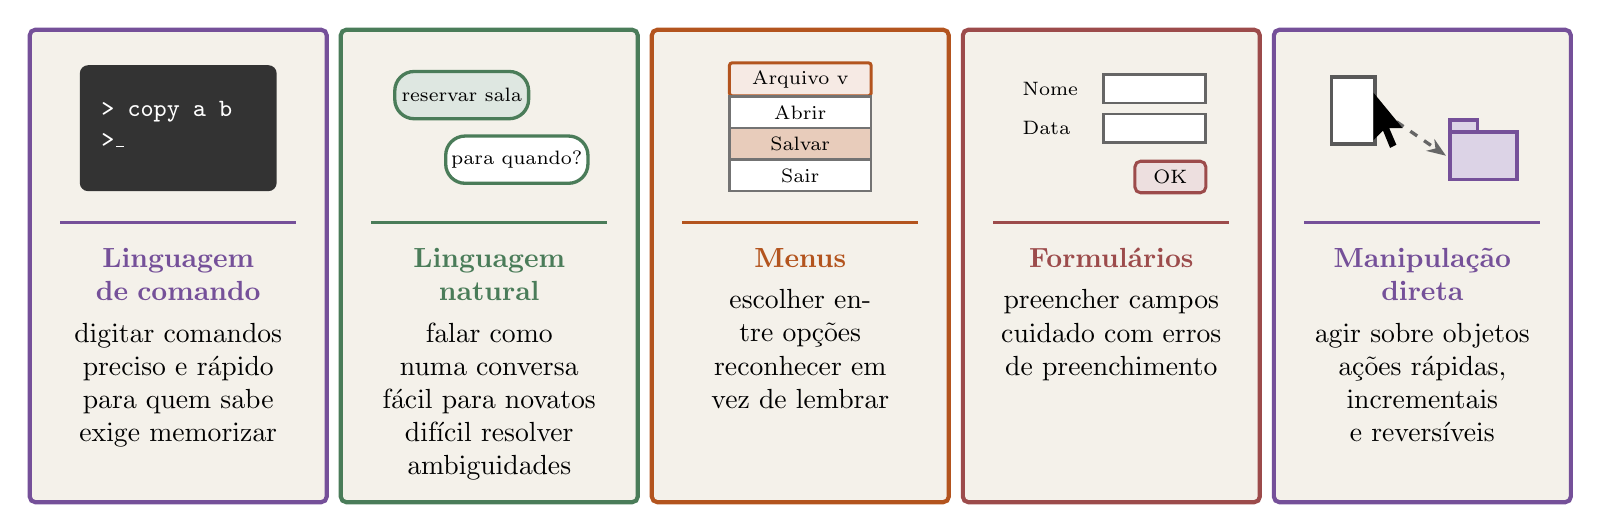
\begin{tikzpicture}[x=1cm,y=1cm]
\node[dbox, draw=dblue, line width=1.5pt, text width=3.35cm, minimum height=6.0cm] at (0.0,0) {};
\draw[dblue, line width=1pt] (-1.5,0.55) -- (1.5,0.55);
\fill[black!80, rounded corners=3pt] (-1.25,0.95) rectangle (1.25,2.55);
\node[white, font=\small\ttfamily, align=left, anchor=west] at (-1.1,1.8) {>\ copy a b\\ >\_};
\node[font=\normalsize, text width=3.1cm, align=center, anchor=north] at (0.0,0.35) {\textbf{\textcolor{dblue}{Linguagem de comando}}\\[3pt] digitar comandos\\ preciso e rápido para quem sabe\\ exige memorizar};
\node[dbox, draw=dgreen, line width=1.5pt, text width=3.35cm, minimum height=6.0cm] at (3.95,0) {};
\draw[dgreen, line width=1pt] (2.45,0.55) -- (5.45,0.55);
\node[dbox, draw=dgreen, fill=dgreen!18, rounded corners=7pt, line width=1.2pt, minimum width=1.7cm, minimum height=0.6cm, font=\scriptsize, inner sep=2pt] at (3.6,2.17) {reservar sala};
\node[dbox, draw=dgreen, fill=white, rounded corners=7pt, line width=1.2pt, minimum width=1.7cm, minimum height=0.6cm, font=\scriptsize, inner sep=2pt] at (4.3,1.35) {para quando?};
\node[font=\normalsize, text width=3.1cm, align=center, anchor=north] at (3.95,0.35) {\textbf{\textcolor{dgreen}{Linguagem natural}}\\[3pt] falar como numa conversa\\ fácil para novatos\\ difícil resolver ambiguidades};
\node[dbox, draw=dorange, line width=1.5pt, text width=3.35cm, minimum height=6.0cm] at (7.9,0) {};
\draw[dorange, line width=1pt] (6.4,0.55) -- (9.4,0.55);
\node[dbox, draw=dorange, fill=dorange!12, rounded corners=1pt, line width=1.1pt, minimum width=1.8cm, minimum height=0.42cm, font=\scriptsize, inner sep=1pt] at (7.9,2.37) {Arquivo v};
\node[dbox, draw=black!55, fill=white, rounded corners=0pt, line width=0.9pt, minimum width=1.8cm, minimum height=0.4cm, font=\scriptsize, inner sep=1pt] at (7.9,1.95) {Abrir};
\node[dbox, draw=black!55, fill=dorange!30, rounded corners=0pt, line width=0.9pt, minimum width=1.8cm, minimum height=0.4cm, font=\scriptsize, inner sep=1pt] at (7.9,1.55) {Salvar};
\node[dbox, draw=black!55, fill=white, rounded corners=0pt, line width=0.9pt, minimum width=1.8cm, minimum height=0.4cm, font=\scriptsize, inner sep=1pt] at (7.9,1.15) {Sair};
\node[font=\normalsize, text width=3.1cm, align=center, anchor=north] at (7.9,0.35) {\textbf{\textcolor{dorange}{Menus}}\\[3pt] escolher entre opções\\ reconhecer em vez de lembrar};
\node[dbox, draw=dred, line width=1.5pt, text width=3.35cm, minimum height=6.0cm] at (11.85,0) {};
\draw[dred, line width=1pt] (10.35,0.55) -- (13.35,0.55);
\node[font=\scriptsize, anchor=west] at (10.6,2.25) {Nome};
\draw[black!60, fill=white, line width=1pt] (11.75,2.07) rectangle (13.049999999999999,2.43);
\node[font=\scriptsize, anchor=west] at (10.6,1.75) {Data};
\draw[black!60, fill=white, line width=1pt] (11.75,1.57) rectangle (13.049999999999999,1.93);
\node[dbox, draw=dred, fill=dred!18, rounded corners=2pt, line width=1.1pt, minimum width=0.9cm, minimum height=0.4cm, font=\scriptsize, inner sep=1pt] at (12.6,1.13) {OK};
\node[font=\normalsize, text width=3.1cm, align=center, anchor=north] at (11.85,0.35) {\textbf{\textcolor{dred}{Formulários}}\\[3pt] preencher campos\\ cuidado com erros de preenchimento};
\node[dbox, draw=dblue, line width=1.5pt, text width=3.35cm, minimum height=6.0cm] at (15.8,0) {};
\draw[dblue, line width=1pt] (14.3,0.55) -- (17.3,0.55);
\draw[black!65, fill=white, line width=1.2pt] (14.65,1.55) rectangle (15.200000000000001,2.4);
\draw[dblue, fill=dblue!25, line width=1.3pt] (16.150000000000002,1.1) rectangle (17.0,1.7);
\draw[dblue, fill=dblue!25, line width=1.3pt] (16.150000000000002,1.7) rectangle (16.5,1.85);
\draw[black!60, dashed, line width=1.2pt, -{Stealth[length=2.4mm]}] (15.3,1.95) -- (16.1,1.4);
\fill[black] (15.180000000000001,2.2) -- (15.180000000000001,1.6) -- (15.3,1.72) -- (15.39,1.5) -- (15.47,1.54) -- (15.38,1.75) -- (15.55,1.75) -- cycle;
\node[font=\normalsize, text width=3.1cm, align=center, anchor=north] at (15.8,0.35) {\textbf{\textcolor{dblue}{Manipulação direta}}\\[3pt] agir sobre objetos\\ ações rápidas, incrementais e reversíveis};
\end{tikzpicture}
\end{document}
